%% This LaTeX-file was created by <skk> Mon May 11 09:37:13 1998
%% LyX 0.12 (C) 1995-1998 by Matthias Ettrich and the LyX Team

%% Do not edit this file unless you know what you are doing.
\documentclass{article}
\usepackage[T1]{fontenc}
\usepackage{a4wide}
\setlength\parskip{\medskipamount}
\setlength\parindent{0pt}
\usepackage{graphics}

\makeatletter


%%%%%%%%%%%%%%%%%%%%%%%%%%%%%% LyX specific LaTeX commands.
\newcommand{\LyX}{L\kern-.1667em\lower.25em\hbox{Y}\kern-.125emX\spacefactor1000}

%%%%%%%%%%%%%%%%%%%%%%%%%%%%%% Textclass specific LaTeX commands.
\newenvironment{lyxcode}
  {\begin{list}{}{
    \setlength{\rightmargin}{\leftmargin}
    \raggedright
    \setlength{\itemsep}{0pt}
    \setlength{\parsep}{0pt}
    \ttfamily}%
   \item[]}
  {\end{list}}

\makeatother

\begin{document}


\title{Detailed product specification}


\author{Group 7}

\maketitle
\tableofcontents

\listoffigures


\section{Design decisions}

The prototype door-entry system is designed to offer the following features:

\begin{itemize}
\item high level of reliability
\item failsafe mechanisms in the event of tamper or power failure
\item simple user interface
\item voice communication in two directions
\item video communication in one direction
\end{itemize}
This has been facilitated by the use of various technologies. The failsafe mechanisms
are provided by the use of a mechanical and electro-mechanical combination of
lock mechanisms. In normal operation, the electro-mechanical door mechanism
operates to unlock the door, while a Yale-type latched doorlock allows manual
operation with a conventional key. This means that, for example, in the event
of system failure due to power supply interruption, access can still be gained
to the property by use of a key. Normally this key would be held by only one
or two people, such as the security staff, and should not be distributed for
widespread use as this would defeat the security features inherent in the electronic
mechanism. 

The main electro-mechanical mechanism is driven by lock control unit, which
in turn is connected by a serial link of variable length to the remote PC. The
lock control unit has the capability to automatically control entry without
needing to communicate with the remote PC, and is therefore protected from failure
in the event of a break in the serial link. 

A simple user interface has been designed, which offers a high degree of reliability
and security. Although magnetic swipe cards are a widely-used and low-cost technology
in door-lock systems, this design does not use them. There is another system
which offers greater reliability and convenience, while still being relatively
low-cost for small to moderate-sized markets. This technology is called iButton
and it is manufactured by Dallas Semiconductor; it consists of a small button-shaped
tag which can be mounted on a laminated identity card or a plastic keyring holder.
This means it is more convenient to carry around than a conventional magnetic
swipe card. 

Additionally, it does not require moving contact for it to be read, and cannot
be wiped by magnetic fields; this technology was therefore chosen to meet the
needs of our chosen market. Each iButton is manufactured with a unique identification
number, which our system reads from the device and uses to identify the user.
The user is then required to enter a Personal Identification Number (PIN) which
then allows them to enter the building. The PIN is entered using a conventional
numeric keypad, which is part of the lock control system. 

The second mode of operation requires the use of video and audio systems. The
design requirement of using a serial link means that this data has to be digitised
and sent over the link. These functions are also carried out by the lock control
unit. It is proposed that the final product would have the entry buzzer button
located just below the camera, so that the picture from the camera would be
of the visitor's face. The location of the microphone and speaker of the audio
system are less important, but these would be part of the same external unit,
and would be separate from the lock control unit itself.

Finally, the design is such that external tampering does not make access possible.
The input devices (camera, keypad, iButton reader, microphone) and output devices
(speaker, status indicators) are wired so that they cannot cause the electro-mechanical
door latch mechanism to activate. As a backup to this, the door position sensor
will detect if the door has been opened without the electronic authorisation
being issued. If this happens, an alarm will sound in the lock control unit
and at the PC; this can be overridden from the PC side.


\section{The door-lock unit hardware}


\subsection{Specific hardware devices }

The door entry system consists of several functional hardware components. These
components provide the interface to the person who is requesting access to the
property. Our hardware interface carries out the following input and output
functions:

\begin{itemize}
\item keypad data input (including the doorbell function)
\item iButton serial number input 
\item intercom audio input 
\item door position detector input 
\item video camera picture input 
\item intercom audio output 
\item door lock control signal output 
\item visual status output (door open, system ready, access denied) 
\end{itemize}
The hardware component of the prototype system is based around a Motorola 68040
prototyping board (IDP), to which we have connected a Connectix Quickcam. In
order to provide the remaining functions we have added an interface board, which
incorporates the keypad, the intercom functions, the door position detector,
the iButton interface, the visual status outputs, and the door lock control. 


\subsection{Detailed interface description}

Component choice was determined by a number of factors. Cost, suitability to
the functional task, simplicity of design and interfacing, and suitability for
prototyping were paramount in the selection process. The use of the 68230, EPLD,
DAC and ADC devices was a direct requirement of the product specification, as
these devices provide the majority of the functionality of the product. In addition,
the design incorporates a number of secondary devices which complement the interfacing
logic and ensure the correct operation of the major components. Finally, the
design uses a keypad encoder to minimise the complexity of the keypad software
routines and hardware connections. This could have been implemented in a custom
logic device, but this was deemed unnecessary as there are good commercial devices
available to do this.

The interface board uses a Motorola 68230 parallel interface device, which gives
a capacity of 24 input or output lines. This device is asynchronous, so it is
connected to the IDP through a state machine, implemented in a single logic
device (an Electronically Programmable Logic Device or EPLD). A D-type flip-flop
is used to synchronise the asynchronous signals from the 68230 with the IDP
clock, as required by the IDP bus specifications. The clock signal for the EPLD
and the flip-flop is derived from the bus clock (6.25MHz) which is doubled using
a phase-lock loop device to 12.5MHz. 

The 68230 device and its associated state machine have been designed to operate
at a clock speed of 10MHz; this clock signal is provided by a separate clock
signal generator device on the interface board. The requirement for tri-state
signals on some of the bus lines has been met by using a tri-state buffer device
on these lines.

The interface functionality is provided by four devices: the Analogue-to-Digital
Converter (ADC), the Digital-to-Analogue Converter (DAC), the iButton interrogation
circuit and the keypad. Each of these systems is described in detail below.
The arrangements for connecting these devices to the 68230 are based on the
allocation of the 24 input/output lines of this device. 8 of these lines have
been allocated to a bi-directional data bus which connects the ADC and the DAC.
In addition, 1 timer line is required to control the rate of sampling.

Another 4 lines have been allocated as inputs for the keypad interface bus;
up to 16 individual keys can be multiplexed onto this. The prototype design
uses a 12 key keypad, so this leaves the possibility of another 4 inputs being
added later; for example a doorbell could be wired in as an extra key. A fifth
input serves as a status line, signalling to the 68230 that a key has been pressed.
This arrangement allow the status of the keypad to be monitored by checking
the state of a single input.

One line has been allocated as a bidirectional line for connection to the iButton
interrogation device. In practice, this output is always low, due to the design
of the interface protocol to the iButton hardware.


\subsection{Data flow within the interface board }

The central component in the interface board is the 68230 device, through which
all the data is passed. The 68230 consists of a set of 32 registers, 3 of which
are mapped to the 24 pins of the bidirectional parallel lines. Another 3 registers
control the direction of the data flow in these lines; by writing to and reading
from these registers, the direction of data movement can be controlled and the
movement of data can be achieved. The 68230 is attached to the first 8 bits
of the IDP bus 32-bit data channel, and the registers are indexed by connection
to address lines A2 to A6. In practice, this means that the 68230 registers
are addressed in steps of 4; this has been done to maintain consistency with
the existing 68230 device on the IDP board.

The bus from the IDP interface to the 68230 is bidirectional, and the data flow
is controlled by the following handshaking signals: 

\begin{itemize}
\item Address Strobe 
\item Slot Address 
\item Read/Write 
\item Reset 
\item Transfer Acknowledge 
\item Cache Inhibit 
\end{itemize}
These signals are managed by the EPLD state machine (see figure \ref{blockdiagram},
page \pageref{blockdiagram}), which generates the necessary signals for the
IDP bus and the 68230 device at the correct times in relation to the bus clock
frequency.

\begin{figure}
{\centering \resizebox*{1\textwidth}{!}{\rotatebox{270}{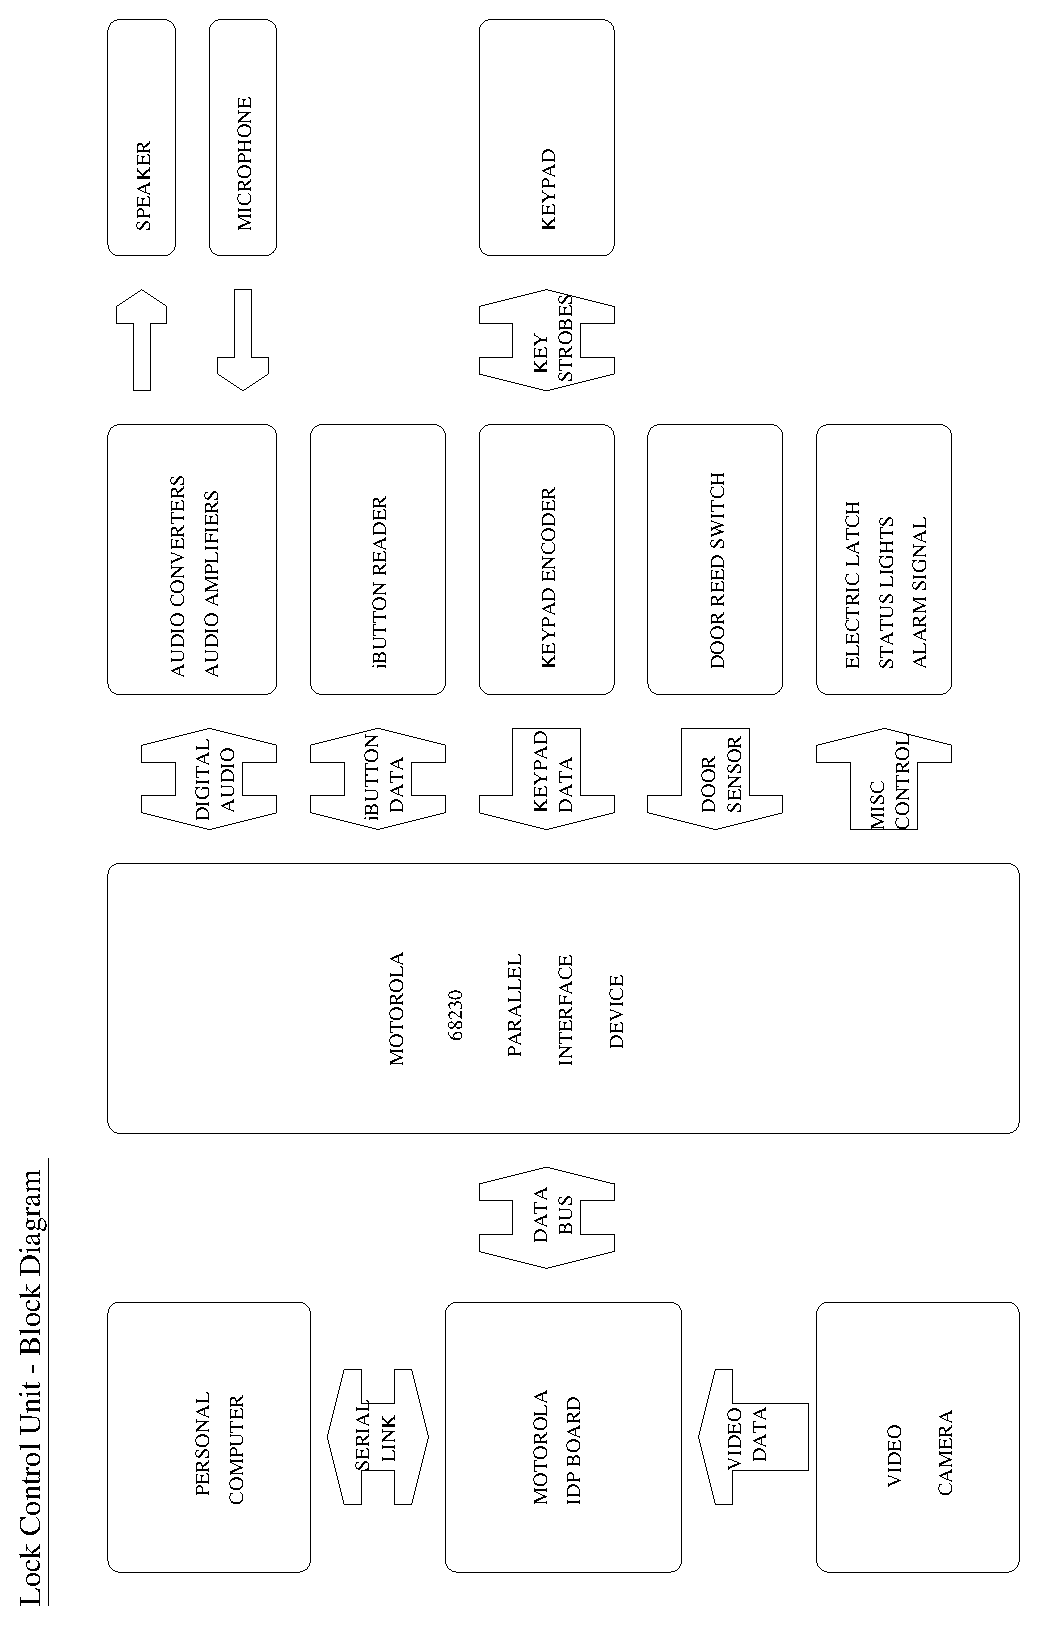
\includegraphics{blockdiag.eps}}} \par}


\caption{\label{blockdiagram}Data transfer block diagram}
\end{figure}

From the 68230 the data flow takes a variety of forms. There is an 8-bit bus
which connects to the ADC and DAC components, and which is bidirectional to
allow reading from and writing to these devices. There is a read-only 4-bit
bus which allows reading of the status of the keypad, and there is a 1-bit bidirectional
bus which allows the interrogation of the iButton device.


\subsection{Hardware construction }

The prototype hardware will consist of three distinct units; the remote PC,
the Motorola IDP board and the IDP interface board. The first two of these are
supplied in assembled form, while the latter will be constructed on prototyping
board. The construction technology used for this will be wire-wrap interconnection,
which allows for rapid development and board reworking in the event of minor
redesigns. The keypad will be mounted on the prototype board as this provides
a stable, flat surface, while the iButton reader, speaker and microphone will
be external components. There will also be connections for the electro-mechanical
latch and the door position sensor. The status indicators will be board-mounted
to minimise the number of external connections.

The custom logic EPLD is programmed from a state diagram (see figure \ref{readtiming},
page \pageref{readtiming}). This ensures that the interface between the 68230
and the IDP bus adheres to the standards given in the IDP documentation (see
figure \ref{writetiming}, page \pageref{writetiming}, for bus timing diagrams).

\begin{figure}
{\centering \resizebox*{1\textwidth}{!}{\rotatebox{270}{\includegraphics{time-read.eps}}} \par}


\caption{\label{readtiming}Read timing diagram}
\end{figure}

\begin{figure}
{\centering \resizebox*{1\textwidth}{!}{\rotatebox{270}{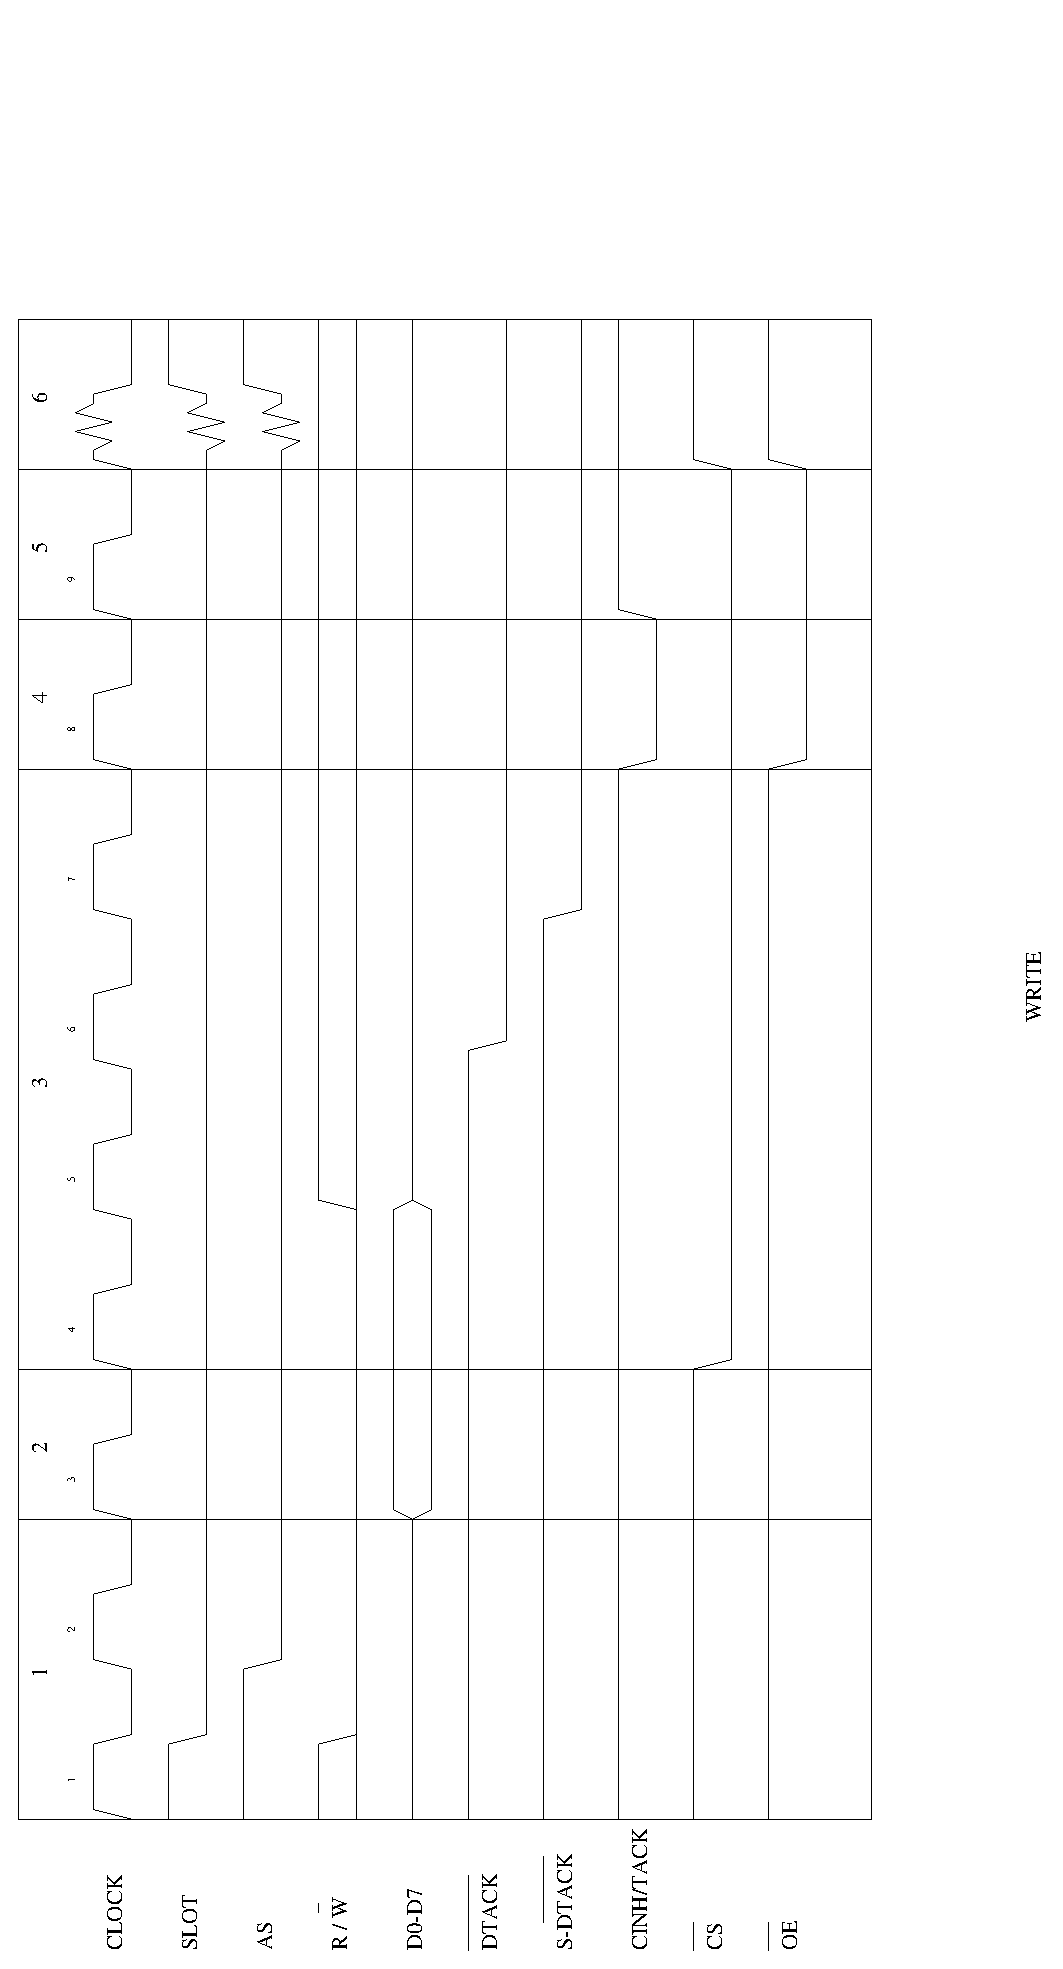
\includegraphics{time-write.eps}}} \par}


\caption{\label{writetiming}Write timing diagram}
\end{figure}\begin{figure}
{\centering \resizebox*{1\textwidth}{!}{\rotatebox{270}{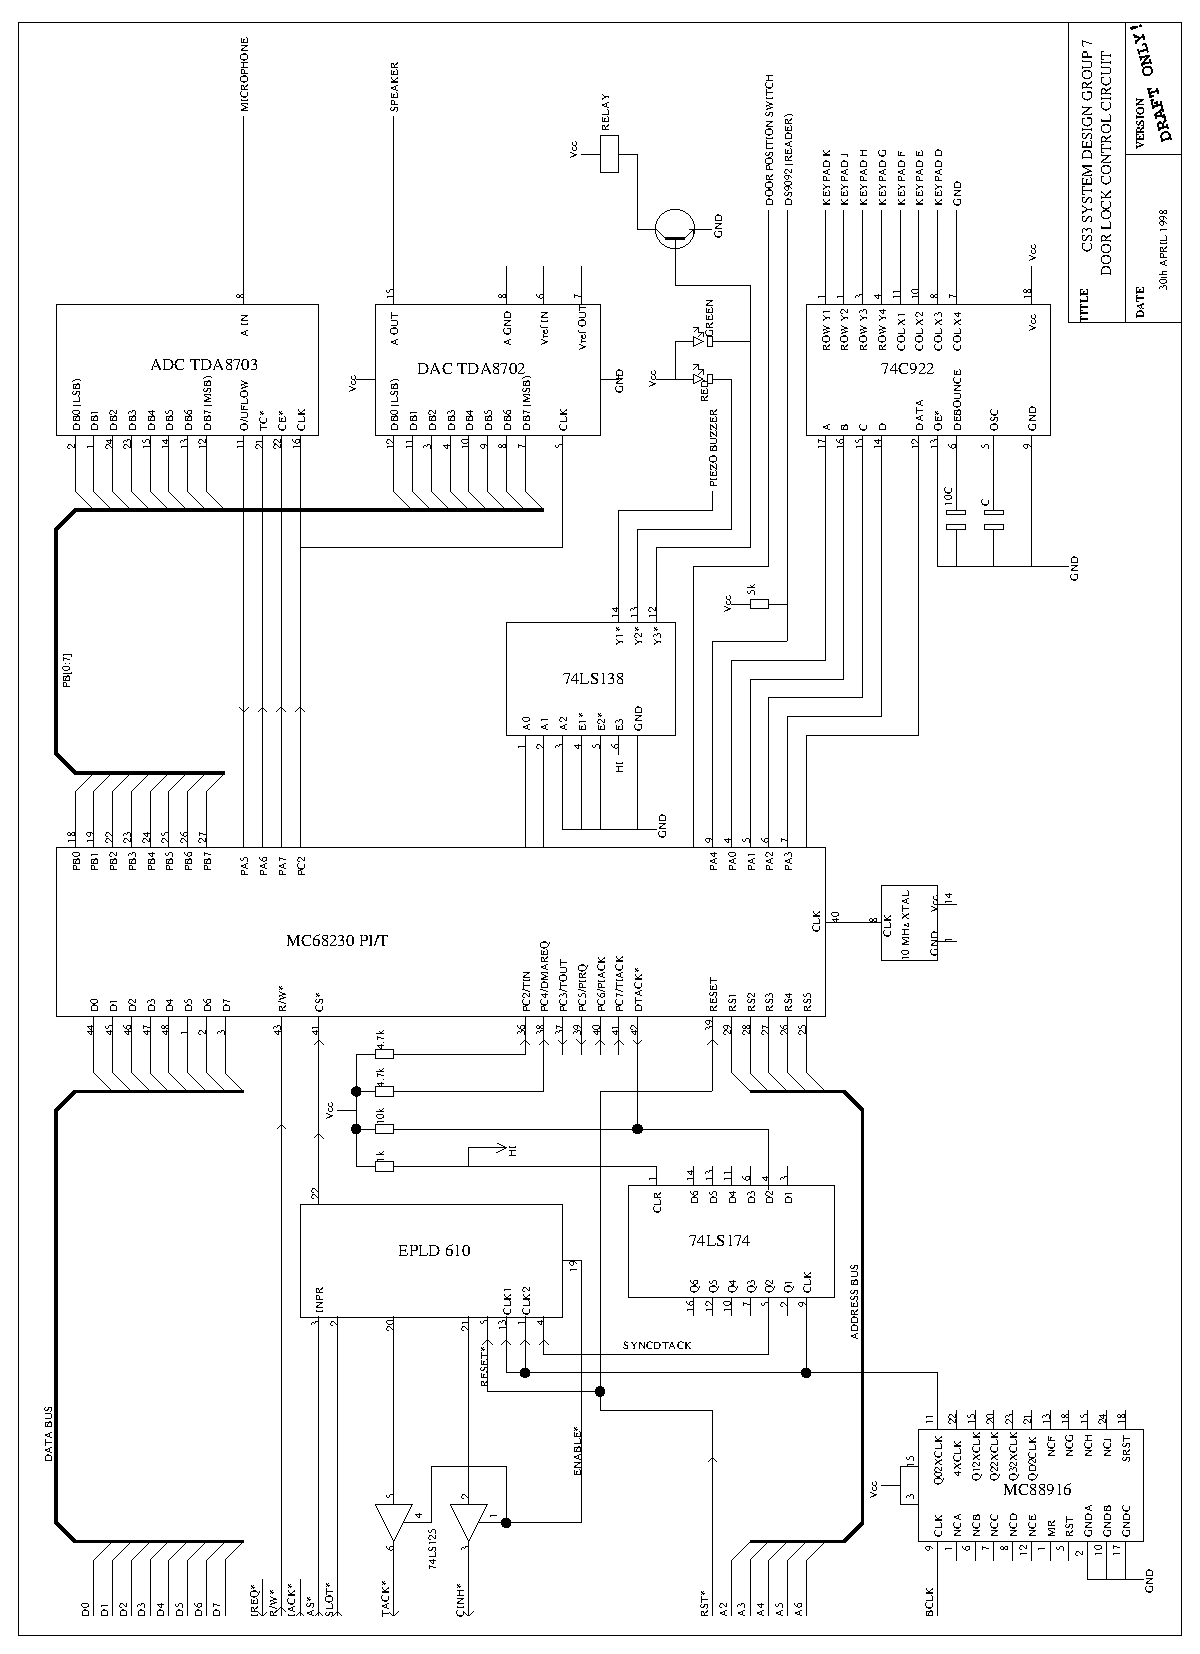
\includegraphics{cctdiag.eps}}} \par}


\caption{Circuit diagram}
\end{figure}


\section{The software}

The software is composed of four components running on two platforms: a daemon
and GUI running on the client (Linux for the prototype), and a program loader
and general control software running on the board (the Motorola IDP). Many support
routines are used, some common to both platforms; these are divided into modules:

\begin{itemize}
\item serial --- provides the communication subsystem; this operates in parallel with
the rest of the software, using interrupts or signals;
\item low-level --- provides functions to access the hardware on the Motorola IDP
board and the secondary board;
\item video --- grabs, compresses and decompresses frames;
\item audio --- samples, compresses, decompresses and plays back audio;
\item control --- handles the database and configuration information, and sends orders
to various sections.
\end{itemize}

\subsection{The Linux software}


\subsubsection{The daemon}

The daemon runs continuously as long as the PC is switched on. It acts as an
intermediary between the Motorola board and the user interface; it also provides
vital functions to the Motorola board to allow the latter to download its software
and the user interface for automatic operation without the user interface being
loaded.

Communication with the Motorola board uses the serial subsystem; data transfers
with the user interface go through the System V IPC shared memory mechanism\footnote{
Note that System V IPC must therefore be compiled in the Linux kernel.
}. A user signal (\texttt{SIGUSR1}) can be sent by either the daemon or the GUI
to indicate that data needs to be transferred.

During normal operation, the daemon stores the last frame taken at any given
time; audio is never transferred without the GUI. When the board indicates the
doorbell has been rung, the daemon activates the GUI, starting it up if necessary,
unless the user has indicated they wish to use the PC without being bothered
by the door-entry software.


\subsubsection{The user interface}

The user interface runs on a Linux PC running the X Windows user interface,
and had been predominantly constructed using the GTK+ toolkit in the C programming
language. It is contained in a binary file together with all other non-continuous
modules such as video and audio. The UI is launched by the daemon on receiving
a message from the Motorola board.

\begin{figure}
{\centering \resizebox*{0.5\textwidth}{!}{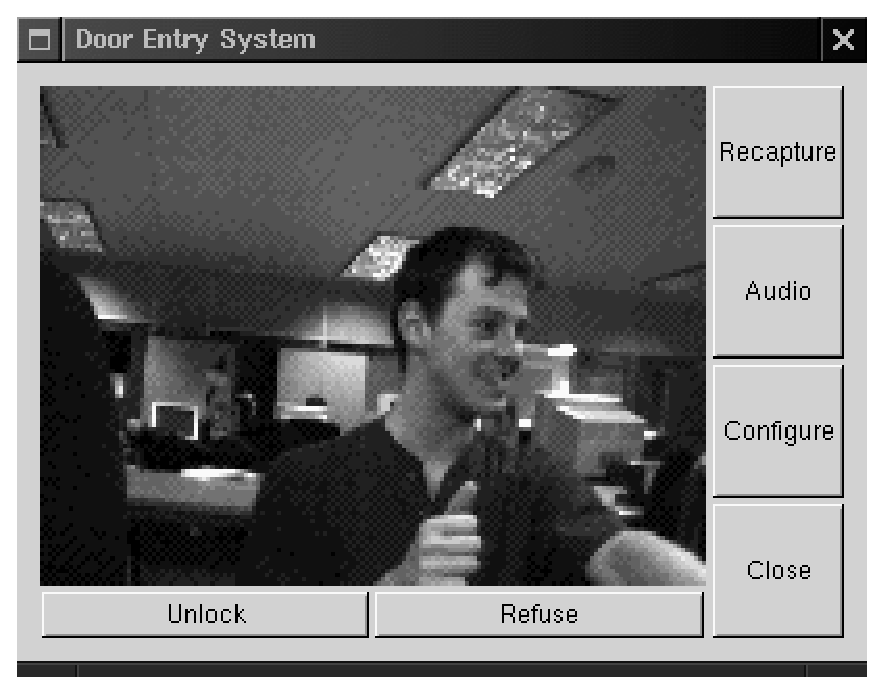
\includegraphics{gui_grab.ps}} \par}


\caption{\label{screenshot1}Screenshot of prototype GUI}
\end{figure}

The main window is shown in fig \ref{screenshot1}, page \pageref{screenshot1}.
If this window is minimised it will be activated whenever someone comes to the
door. Normally the video frames will be updated approximately once every second
and there will be no audio. When someone presses the buzzer and the PC user
reacts, two way sound transmission will begin and continue until a (long) timeout
expires, or the person is accepted or rejected. The functions of the various
buttons are as follows:

\begin{itemize}
\item recapture --- pressing this button transmits a request to the Motorola board
to recapture a frame of video;
\item unlock --- this causes the door to unlock;
\item refuse --- this denies entry;
\item audio --- this loads an audio configuration program (mixer);
\item config --- this opens the system configuration panel;
\item close --- this closes the interface window;
\item do not disturb (not present in the screenshot) --- this minimises the interface
window and tells the daemon no to pop it up.
\end{itemize}

\subsection{The Motorola software}


\subsubsection{The initial program loader}

This piece of software sits in a tight polling loop waiting for the client to
activate; it then proceeds to download the board software into memory and transfer
control to it. It is burnt into a PROM and automatically loaded when the board
is switched on.


\subsubsection{The board control software}

This implements the board-side of the door-entry system in software. It interacts
with the hardware on the boards, and communicates with the client.

\begin{figure}
{\centering \resizebox*{1\textwidth}{!}{\rotatebox{270}{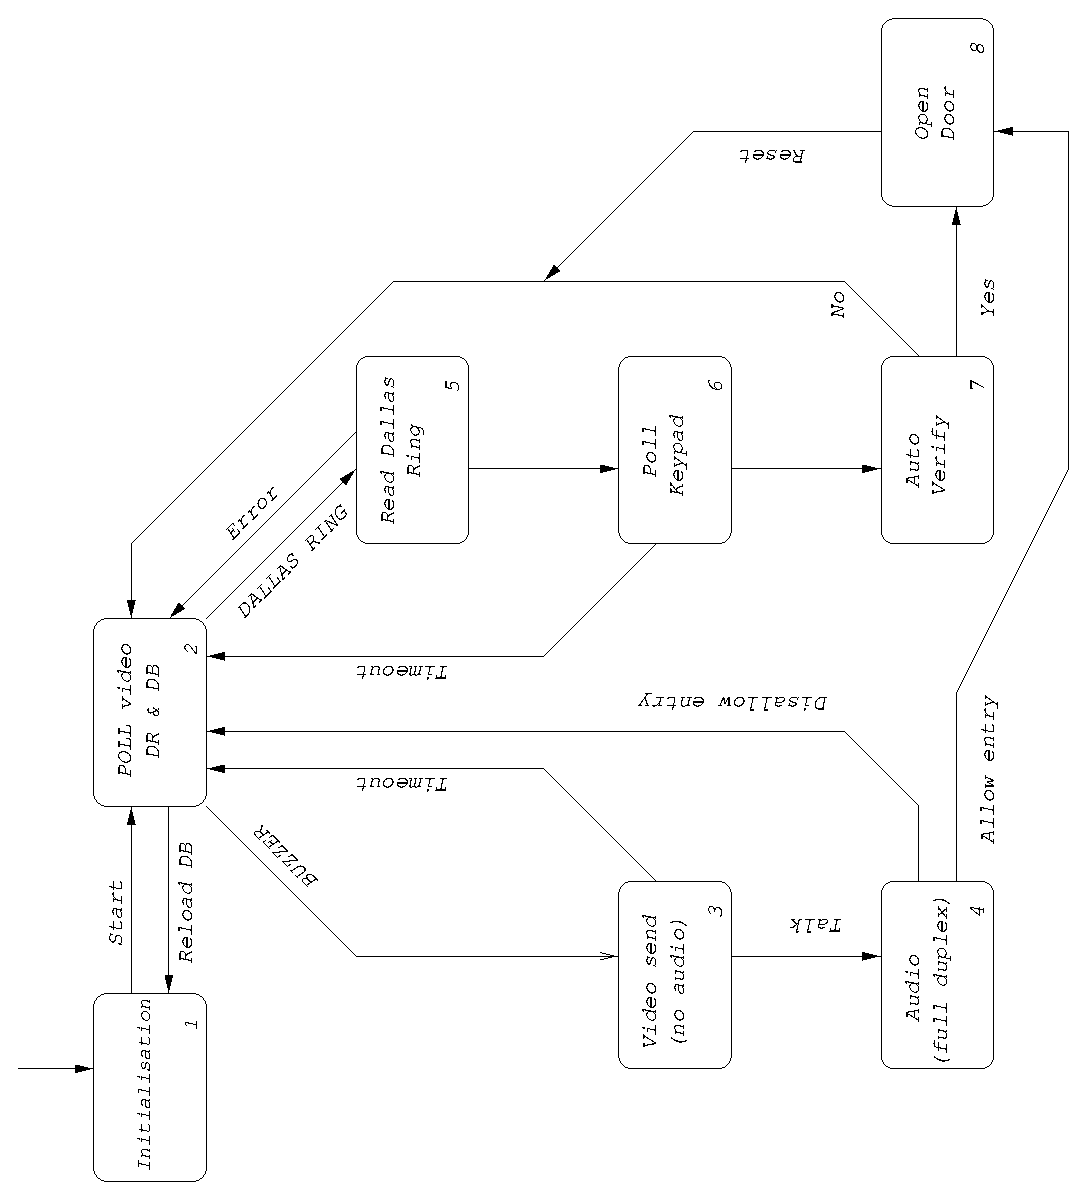
\includegraphics{board_flowchart.eps}}} \par}


\caption{\label{Motorola state diagram}Motorola software state diagram}
\end{figure}The Motorola software state diagram (figure \ref{Motorola state diagram}, page
\pageref{Motorola state diagram}) gives an overview of the operation of this
software. The program can be in one of eight states at any given time, and certain
well defined circumstances cause it to move from one state to another. In the
diagram, rounded boxes represent states, and arrows represent transitions; the
text on the arrows gives an indication of the condition which provokes the transition.
Communication between states is achieved through global flags.


\paragraph{State 1 --- Initialisation}


\subparagraph{Functional description}

This state will:

\begin{itemize}
\item initialise the serial transport subsytem;
\item retrieve configuration information from the client;
\item retrieve the user database from the client;
\item initialise the hardware subsystems using their initialisation functions.
\end{itemize}

\subparagraph{Transitions}

State 2 will be entered upon completion of the above.


\subparagraph{Communications to the client}

Configuration information and the database are requested from the client's control
module using the \texttt{CONTROL} tag (more specifically with the \texttt{REQUEST\_CFG}
and \texttt{REQUEST\_DB} sub-tags).


\subparagraph{Communications from the client}

The above information is transferred using \texttt{CONTROL} tags (\texttt{DATA\_CFG}
and \texttt{DATA\_DB}).


\subparagraph{Support used}

This states makes use of all the support modules --- it needs serial to communicate,
control to store the configuration and database, and it has to initialise everything.


\paragraph{State 2 --- Normal operation}


\subparagraph{Functional description}

This state performs four functions: 

\begin{itemize}
\item it polls the video camera, it captures an image and uses a combination of frame-difference
and RLE encoding to compress the image before sending it via serial to the Linux
client machine;
\item it polls the iButton to detect whether a ring is present in the detector;
\item it checks for a signal from the client;
\item it polls the buzzer (linked to the keypad).
\end{itemize}

\subparagraph{Transitions}

The following states can be entered from state 2:

\begin{itemize}
\item state 1 --- a signal is received from the client instructing the board to enter
the initialisation state;
\item state 3 --- the buzzer is pressed;
\item state 5 --- an iButton is detected.
\end{itemize}
Otherwise state 2 will loop.


\subparagraph{Communications to the client}

Compressed frames from the video camera are sent to the video module using the
\texttt{VIDEO} tag.


\subparagraph{Communications from the client}

The client can request a transition to state 1 using the \texttt{CONTROL} tag
(\texttt{RESET} sub-tag).


\subparagraph{Support}

This state uses the control, low-level and video modules.


\paragraph{State 3 --- Wait for PC user to respond}


\subparagraph{Functional description}

This state informs the client that the buzzer has been pressed. It then continues
to transmit video until it times out (according to a preset timeout value) or
the client acknowledges the buzzer. 


\subparagraph{Transitions}

The following states can be entered from state 3:

\begin{itemize}
\item state 2 --- the timeout expires (\emph{i.e.} the client fails to respond);
\item state 4 --- the client responds to the buzzer signal.
\end{itemize}
Otherwise state 3 will loop.


\subparagraph{Communications to the client}

A \texttt{CONTROL} message (\texttt{BUZZER} sub-tag) informs the client that
the buzzer has been pressed.


\subparagraph{Communications from the client}

A \texttt{CONTROL} message (\texttt{BUZZER\_ACK} sub-tag) acknowledges receipt
of the \texttt{BUZZER} signal.


\subparagraph{Support}

This state makes use of the control and video modules.


\paragraph{State 4 --- Conversation with the visitor}


\subparagraph{Functional description}

State 4 is the state which handles the audio when there is someone at the door.
It samples from the microphone at the door, compresses the data and sends it
to the PC. It also takes compressed samples from the PC and plays them via the
speaker at the door. Additionally, the system must check for input from the
PC user, so that they can choose to grab some more video, open the door, or
refuse entry.


\subparagraph{Transitions}

The following states can be entered from state 4:

\begin{itemize}
\item state 2 --- the client refuses entry, or the timeout expires;
\item state 8 --- the client authorises entry.
\end{itemize}
Otherwise state 4 will loop.


\subparagraph{Communications to the client}

\texttt{AUDIO} messages transmit audio to the audio module; \texttt{VIDEO} messages
can also be used to transmit video.


\subparagraph{Communications from the client}

\texttt{AUDIO} messages transmit audio; \texttt{CONTROL} messages indicate the
user's response (\texttt{AUTHORISE} or \texttt{REJECT}) or a request for more
video (\texttt{GRABFRAME}).


\subparagraph{Support}

This state uses the control, low-level and audio modules.


\paragraph{State 5 --- Read the iButton}


\subparagraph{Functional description}

This state is entered when a iButton is present in the reader; it reads the
64 bits of information off the ring and stores them in a buffer for later use.


\subparagraph{Transitions}

The following states can be entered from state 5:

\begin{itemize}
\item state 6 --- the information was successfully read;
\item state 2 --- an error occurred during the read.
\end{itemize}

\subparagraph{Communications to the client}

A \texttt{CONTROL} message (\texttt{USERID}) will be sent to allow the auto
alert window to display information about the visitor.


\subparagraph{Support}

This state uses the control and low-level modules.


\paragraph{State 6 --- Retrieve PIN}


\subparagraph{Functional description}

This state attempts to read a PIN from the keypad, by repeatedly polling it
until either a full PIN is read, or the timeout expires.


\subparagraph{Transitions}

The following states can be entered from state 6:

\begin{itemize}
\item state 7 --- a PIN is successfully read;
\item state 2 --- the timeout expires.
\end{itemize}

\subparagraph{Support}

This state uses the low-level module only.


\paragraph{State 7 --- Verify user ID and PIN}


\subparagraph{Functional description}

This state verifies the authenticity of the user wishing to gain entry. It looks
at the UID and PIN read by previous states and stored in memory, compares these
with entries in the database, and decides whether to authorise or reject the
visitor. The outcome is sent to the client for logging.


\subparagraph{Transitions}

The following states can be entered from state 7:

\begin{itemize}
\item state 8 --- the user ID is in the database and the PIN is correct;
\item state 2 --- the user ID isn't in the database, or the PIN is incorrect.
\end{itemize}

\subparagraph{Communications to the client}

A \texttt{CONTROL} message (\texttt{LOG\_ENTRY}) informs the client of the outcome
of the verification.


\subparagraph{Support}

This state uses the control module.


\paragraph{State 8 --- Open door}


\subparagraph{Functional description}

This state opens the door.


\subparagraph{Transitions}

State 2 will be entered once the door is opened.


\subparagraph{Communications to the client}

A \texttt{CONTROL} message (\texttt{DOOR\_OPEN}) indicates the door was opened.


\subparagraph{Support}

This state uses the control and low-level modules.


\subsection{The secondary board support software (``low-level'' module)}

These functions provide the interface to the secondary board, and to some features
of the IDP board.


\subsubsection{The iButton reader}

The iButton reader is accessed through the MC68230 on the secondary board, using
the bus. A signal can be sent to it to determine whether a ring is present;
if one is, the ring can be told to transmit its contents using a well-defined
protocol.

Two functions and a structure are provided to access information on the ring.
The structure is defined as follows:

\begin{lyxcode}
typedef~struct

\{

~~unsigned~char~product;

~~unsigned~char~id~{[}6{]};

~~unsigned~char~crc;

\}~ringinfo;
\end{lyxcode}
The functions are:

\begin{itemize}
\item \texttt{int~checkring~(void)} --- returns 1 if a ring is present, 0 otherwise;
\item \texttt{ringinfo~{*}~getringinfo~(void)} --- retrieves the ring's information
and places it in a structure.
\end{itemize}

\subsubsection{The keypad}

The keypad is accessed through the MC68230 controller. The doorbell is wired
through the keypad, as well as the standard keys. Again, a signal can be sent
to determine whether a key is currently being pressed; then its value can be
read. Obviously when polling the keypad it is necessary to ensure that the key
has been released before waiting for a new keypress.

Two functions are provided:

\begin{itemize}
\item \texttt{int~checkkeypad~(void)} --- returns 1 if a key is being pressed, 0 otherwise;
\item \texttt{unsigned~char~getkeypad~(void)} --- returns the value of the key being
pressed; this is an integer between 0 and 12, 0--9 corresponding to the digits
0--9, \texttt{KP\_STAR} to the star symbol, \texttt{KP\_HASH} to the hash symbol,
and \texttt{KP\_DOORBELL} to the doorbell.
\end{itemize}
Note that initially one of the auxiliary keys (star or hash) may be used instead
of an actual doorbell.


\subsubsection{The ADC and DAC}

The ADC and DAC are accessed through the MC68230 controller. The ADC samples
its input every time its clock signal fires, and stores the result in an on-board
register which can be queried; the DAC generates the sound corresponding to
any input it receives using a special trigger signal.

Two functions are provided:

\begin{itemize}
\item \texttt{unsigned~char~getsample~(void)} --- returns the current sample from
the ADC;
\item \texttt{void~setsample~(unsigned~char)} --- sends a sample to the DAC.
\end{itemize}

\subsubsection{The NVRAM and RTC}

The NVRAM (non-volatile memory) and RTC (real-time clock) are stored on a memory-mapped
chip on the Motorola board.

The following structure stores time information:

\begin{lyxcode}
typedef~struct

\{

~~unsigned~char~seconds;

~~unsigned~char~minutes;

~~unsigned~char~hours;

~~unsigned~char~day;

~~unsigned~char~date;

~~unsigned~char~month;

~~unsigned~char~year;

\}~rtctime;
\end{lyxcode}
Their precise meaning (with regard for example to the \texttt{year} field) is
up to the programmer, but the values stored in the RTC will be updated automatically.

The following functions access the RTC:

\begin{itemize}
\item \texttt{rtctime~getrtctime~(void)} --- retrieves the current time from the RTC;
\item \texttt{void~setrtctime~(rtctime)} --- stores new data in the RTC.
\end{itemize}
The programmer can use 760 bytes in NVRAM, and these are accessed using the
following functions:

\begin{itemize}
\item \texttt{unsigned~char~{*}~getnvram~(int,~int)} --- returns the data stored in
the given range;
\item \texttt{void~setnvram~(unsigned~char~{*},~int,~int)} --- stores the data in
the given range.
\end{itemize}
The range is specified as going from the first integer argument to the second,
inclusive; so for example \texttt{setnvram~(\&data,~0,~759)} would fill the
whole NVRAM.


\subsubsection{The LED display}

The memory-mapped, 7-segment LED display on the IDP can be accessed using the
\texttt{void~leddisplay~(int)} function, which display the given hexadecimal
digit or blanks the LED if -1 is given as an argument.


\subsubsection{The door}

The door lock's status can be verified and changed using:

\begin{itemize}
\item \texttt{int~getdoorstatus~(void)} --- returns 0 if the door is closed, 1 if
it's open;
\item \texttt{int~opendoor~(void)} --- opens the door, returning 0 in case of success,
-1 in case of failure.
\end{itemize}

\subsubsection{The jiffies counter}

A global variable, defined as

\begin{lyxcode}
unsigned~int~jiffies
\end{lyxcode}
is updated regularly (the exact interval to be used hasn't yet been determined),
using the UART's counter. This can be used as a precise measure of elapsed time.


\subsection{The serial subsystem}


\subsubsection{External interface}

The serial interface is designed to be the same on both the Linux and Motorola
sides of the system. The subsystem transmits packets of data between the two
platforms; these can be of any length (up to four gigabytes).

A data packet, as supplied to and by the serial functions, has the following
structure:

\begin{lyxcode}
typedef~struct

\{

~~unsigned~char~datatype;

~~unsigned~int~length;

~~unsigned~char~{*}~data;

\}~packet;
\end{lyxcode}
The datatype is used by handler functions at the receiving end; the serial subsystem
maintains a programmer-controlled list of handlers, and upon receiving a complete
packet, calls the relevant handler. Two datatypes are predefined by the serial
subsystem though: 0 corresponds to the default handler, used when no handler
is defined for the datatype of a packet, and 1 is the PING packet, used to check
whether the system is alive. The first of these can be redefined by the programmer.

The data pointed to is copied immediately, so that the supplying function needn't
keep a copy. Likewise, receiving functions should copy the data immediately...

The functions defined are as follows:

\begin{itemize}
\item \texttt{int~serialinit~(void)} --- initialises the serial subsystem;
\item \texttt{int~serialclose~(void)} --- closes the serial subsystem;
\item \texttt{int~senddata~(packet~{*})} --- queues a packet (pointed to by the argument);
\item \texttt{int~registerhandler~(unsigned~char,~packethandler)} --- registers a
function which will be called with any incoming packet containing data of the
type given in the first argument;
\item \texttt{int~unregisterhandler~(unsigned~char)} --- removes any handler previously
defined for the given data type; if the default data handler is removed, the
system reverts to the supplied default handler which discards any incoming packets
apart from the PING packet;
\item \texttt{int~ping~(void)} --- checks to see whether the opposite member of the
link is still responding.
\end{itemize}

\subsubsection{Implementation}

The implementation of the serial subsystem on both platforms is event-based.
Queues of incoming and outgoing data are maintained, and whenever the UARTs
are ready to send or receive data is fed to (if there is any outgoing data)
or read from them. The queues are big enough for data overflow never to be a
problem, at least with essential data; if there's no room for a video frame
for example it can just be dropped, but control packets must be transmitted
at all costs.


\paragraph{Common sections}

The event-handling function is \texttt{void~serialevent~(void)}, which is called
whenever the UART signals it's ready to transmit or receive; it then determines
which direction data is needed for, and transfers it to and from the queues.

A 32768-byte buffer stores the incoming data until a complete packet is received,
as determined by the length descriptor. Whenever a complete packet is formed,
the corresponding handler is called, and the buffer can then be re-used.

Output data is stored in a circular, 65536-byte buffer as a stream of raw bytes
which need sent out. When a packet is received, its contents are simply added
to the buffer.


\paragraph{Linux specifics}

The Linux code communicates with the serial port by using the \texttt{ttyS0}
terminal device. Events are provided using the \texttt{IO} signal; a call to
\texttt{select(2)} is then used to determine whether the UART is ready to transmit
or receive. \texttt{serialevent} is called by \texttt{void~iosighandler~(int)},
which is registered as the \texttt{SIGIO} handler. \texttt{termios} functions
are used to set the communications port up.


\paragraph{Motorola specifics}

On the Motorola, access to the UART is done directly since the MC68681 is memory-mapped
and there is no operating system. The PIT (MC68230) is also used since the UART's
IRQ line goes through it. The assembler function \texttt{serialirq} is set up
to handle the UART IRQ exception; it simply calls \texttt{serialevent}.


\subsection{The audio module}

The audio module provides functions to retrieve a compressed sample and to play
back a compressed sample. All the audio functionality is internal to state 4.


\subsubsection{Compression}

The audio compression system is based around ADPCM compression, and takes the
audio down from 8 bits per sample to 2 bits per sample. With an 8kHz sampling
rates this reduces the bandwidth requirements from 64kbps to 16kbps.

The ADPCM compression standard is defined in the CCITT G.726 16kpbs audio compression
standard. G.726 specifications are available from the ITU Web site (www.itu.ch).
The code is taken from Sun Microsystem's implementation, which has been released
into the public domain.


\subsubsection{Format of the data from the hardware}

On the client, the system uses the Open Sound System (OSS) which is part of
the Linux kernel. On the board, sound is taken directly from the 8-bit ADC,
or fed into an 8-bit DAC. In all cases data is an unsigned, 8-bit sample (0
to 255) at 8kHz. 


\subsubsection{Communications}

For the data to be compressed, it first has to be converted to a signed 8-bit
sample (\( -128 \) to 127), then bit-shifted into a 14-bit word for the ADPCM
encoder to work on. Decompression feeds the 2-bit code into the ADPCM decoder
and transforms the resulting 14-bit word into an 8-bit sample.

The 2-bit codes are transported as compactly as possible, \emph{i.e.} four per
byte, in quarter-second packets of approximately 500 bytes.


\subsection{The video module}

This provides functions to retrieve, compress and decompress a frame.


\subsubsection{Format of image as received from video camera}

The image returned from the camera is an array of 19200 bytes. Each of these
has a value between 0 and 15 (therefore only the lower 4 bits of each byte are
used). Each byte represents one pixel of the image. After translation\footnote{
The original data represents black as 0, white as 1, and gray-scales from white
to black respectively as values from 2 to 15.
}, 0 represents black and 15 represents white, intermediate values represent
grey values increasing in lightness as their value increases. The first 160
bytes represent the first horizontal line of the image, and subsequent sub-arrays
of 160 bytes represent subsequent lines of the image.


\subsubsection{Compression algorithm}

The last frame grabbed is always stored locally, so that a logical exclusive
or can be preformed between it and the new frame; the default last frame is
all zero (black). The result of this is that pixels of the image which remain
constant between the two frames become black.

The resulting frame difference image is then scanned using a Run Length Encoding
(RLE) algorithm prior to transmission.


\subsubsection{Format of Run Length Encoded data}

\noindent The Run Length Encoded file should be treated as a stream of 5 bit
blocks. 

The first bit of the block determines it's nature. If the first bit is 0 then
the subsequent 4 bits represent the colour of an individual pixel. If the first
bit is 1 then the subsequent 4 pixels represent the colour of a pixel, and the
subsequent block represents the number of pixels of that colour (minus two,
since we never encode a run of zero or one pixel).


\subsection{The control module}

The control functions handle user authentication and database storage. Functions
are provided to access and modify the user database on the PC, and to transfer
the database to the Motorola board --- it's stored in RAM on the board whenever
the Motorola is switched on, and only downloaded again when it changes. A single
function takes a user ID and PIN and validates it against the database.

The control module also has a \texttt{CONTROL} handler for the communications
subsystem, but this can be replaced by individual states' own handler, for instance
to allow a change of state to be requested. Various control tokens are defined
and refine the \texttt{CONTROL} packet; the states are well enough constrained
for it to be possible for handlers to ignore tokens they don't know.

\end{document}
